\documentclass[11pt]{article}
\usepackage{graphicx}
\usepackage{adjustbox}
\usepackage{dcolumn} 
\usepackage{subcaption}
\usepackage{parskip}
\usepackage{float}
\usepackage[
backref=biber,
style=authoryear,
]{biblatex}
\addbibresource{C:/Users/Ava/Documents/LaTeX/library.bib}
\usepackage[
hidelinks, 
pdfpagelabels=true,
plainpages=false,
colorlinks=false,
bookmarks=true,
pdfview=FitB]{hyperref} % Required for the hyperlinks within the PDF

%opening
\title{What is learned during statistical learning? }
\author{Ava Kiai, Lucia Melloni}
\date{}

\begin{document}

\maketitle

\begin{abstract}

\end{abstract}

\tableofcontents

\section{Introduction}
Statistical learning (SL) is one mechanism by which the brain is able to parse 
continuous streams of sensory information, based on simple statistical features 
alone. \cite{Dehaene2015} SL paradigms have shown the brain to be surprisingly 
effective at detecting statistical regularities in highly impoverished or artificial 
inputs, leading to a discrimination of meaningful boundaries where previously 
none were discernible. \cite{Pelucchi2009, RichardN.Aslin1998, Turk-Browne2005, Turk-Browne2008}

Statistical learning is canonically measured using an explicit word discrimination 
task after exposure to the continuous speech stream. 

Several online statistical learning measures have been previously shown to be 
effectively modulated by implicitly-acquired knowledge of the statistical regularity 
of reoccurring syllables. 

We investigated whether dynamic online measures of statistical learning are able to 
predict performance in the canonical offline task. In a first experiment, we 
implemented a target detection task to measure SL online and an offline explicit 
word recognition task. In a second study, we asked participants to perform the 
online target detection task to further explore the informative capacity of this 
task, in both a structured and random condition.

\section{Experiment 1}
\subsection{Method}
41 individuals participated in the study (x female, mean age, +- sd). Two participants 
were removed from the data pool due to technical failure. Of the 39 remaining
datasets, 33 were used in analyzing the target detection task (one participant failed 
to follow instructions, and technical issues caused partial data loss for the other 
five). However, technical failures in our program were limited to the current task 
being run. Thus, we used data from 38 participants in analyzing the word recognition 
task (data from one participant was overwritten).  

\subsection{Results}
To replicate findings that showed graded reaction times in response to syllables in 
different ordinal positions, we ran a generalized linear model with reaction time (in 
seconds) as outcome variable, fitted with a gamma function and log link function. % cite R lme4 package
Our full model included both ordinal position and block as fixed effects factors, and 
subject as random intercept random effects factor. This model was compared with a lesser
model in which only ordinal position was input as a fixed effect. The lesser model provided
a better fit of the data, with a lower AIC (-6389.2) value and significantly lower deviance 
(-6399.2, ${\chi}^{2}$(21, N = 33) = 49.066, \textit{p} = 0.00049). (See ~\ref{table:Table 2} for regression
results.)
% X2 (degress of freedom, N = sample size) = chi-square statistic value, p = p value.
We also compared both the fuller and the lesser models with random slopes in the random effects
term, but the lesser model with only varying random intercepts in the random effects term still
proved a better fit for observed data (see Table 1. Model output the random slopes fuller model not shown; lesser vs. fuller random slopes models deviance was -6624.3 and -6678.3, respectively; 
${\chi}^{2}$(21, N = 33) = 54.025, \textit{p} < 0.0001). Thus, we conducted further analysis on
results of the lesser model. 

We found that reaction times are modulated by ordinal position such that RTs to word-initial syllables
are notably slower than those to word-medial and word-final syllables. (~\ref{fig:Fig. 1}) We conducted pairwise comparisons on estimated marginal means for levels of the factor 
position with Tukey adjustment, to explore the drop in reaction times between each positions 
(See ~\ref{table:Table 1}). The predicted coefficients from the winning model accurately
reflected the pattern of graded reaction times in the raw data (~\ref{fig:Fig. S1}).

\begin{figure}[H]
	\begin{subfigure}[]{\linewidth}
		\centering
		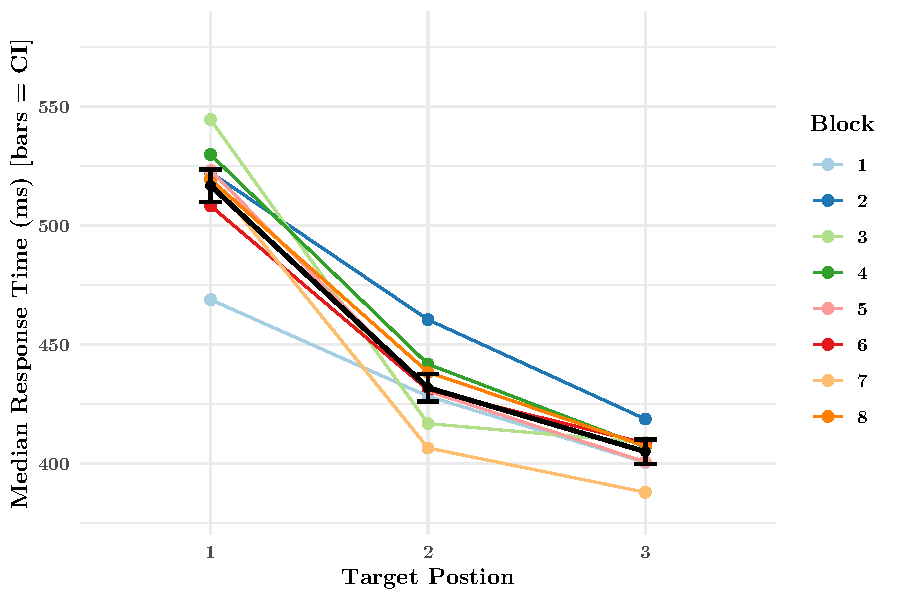
\includegraphics[width=\textwidth]{exp3fig1a.pdf}
		\caption{Ordinal Position of target syllable predicts reaction time. }
	\end{subfigure}
	\newline
	\begin{subfigure}{.5\textwidth}
		\centering
		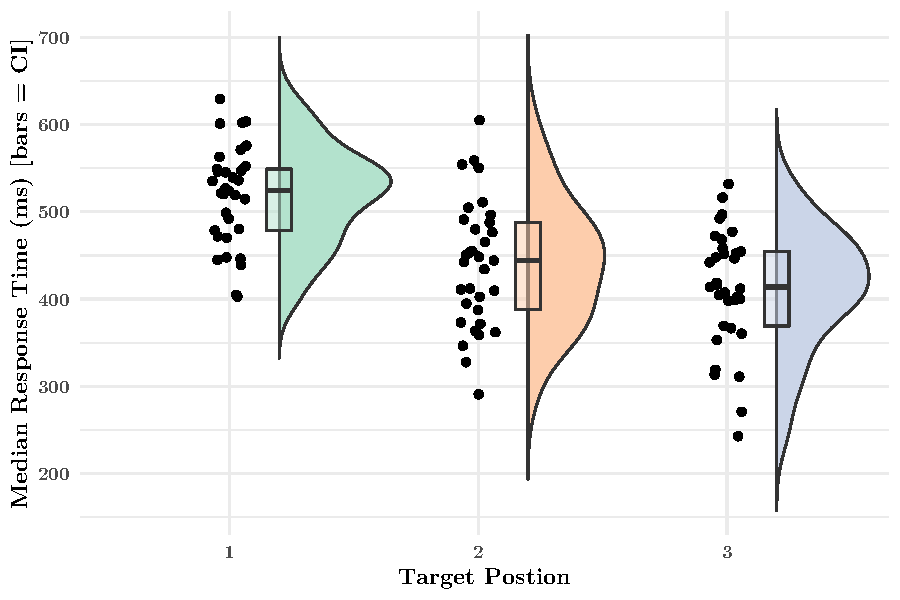
\includegraphics[width=\linewidth]{exp3fig1b.pdf}
		\caption{Averaged over blocks.}
	\end{subfigure}
	\begin{subfigure}{.5\textwidth}
		\centering
		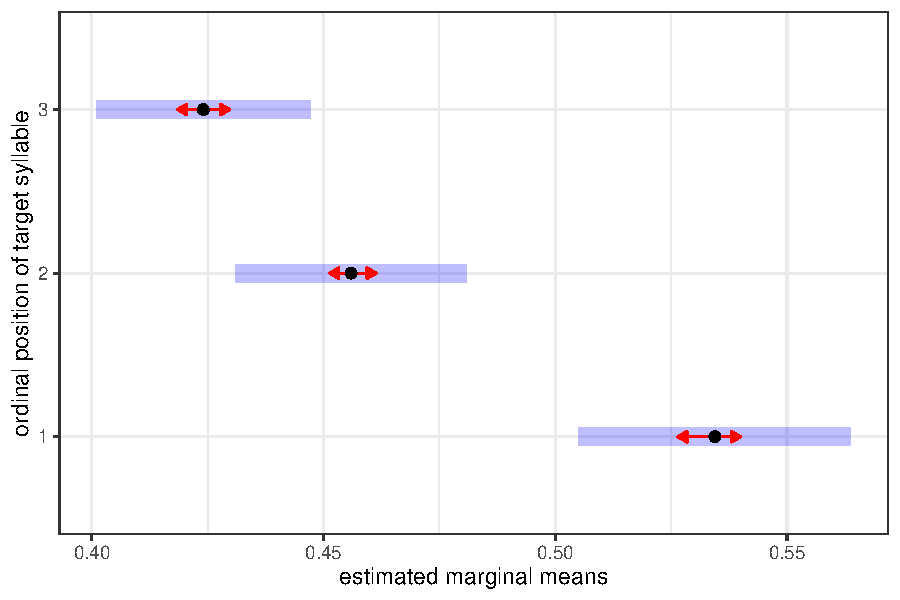
\includegraphics[width=\linewidth]{exp3fig1c.pdf}
		\caption{Contrast of estimated marginal means. }
	\end{subfigure}
	\label{fig:Fig. 1}
\end{figure}

To improve interpretability of the results, we also computed s-values
for each p-value. The s-values is a metric of self-information, or surprisal information measure. 
It can assist in the interpretation of p-values by providing an intuitive transformation of the 
p-value, taking the negative log of the p-value: -$\log_{2}$(\textit{p}). A value of 0 (\textit{p} = 1) is % cite Greenland 2019
perfectly unsurprisingly and surprisal increases exponentially as \textit{s} approaches zero. 
Thus, \textit{S} becomes a measure of information in bits against the null hypothesis. The difference
in means between positions 1 and 3 can be quantified in roughly 139.3 bits. If the null hypothesis of
no difference in means is true, this result is as surprising as getting all heads in 140 fair
coin tosses (\textit{s} rounded to the nearest integer). 

\begin{table}[H] \centering 
	\caption{Contrasts for ordinal positions of target syllables.} 
	\label{table:Table 1} 
	\begin{tabular}{@{\extracolsep{5pt}} ccccccc} 
		\\[-1.8ex]\hline 
		\hline \\[-1.8ex] 
		contrast & estimated marginal diff. & SE & df & z ratio & p value & s value \\ 
		\hline \\[-1.8ex] 
		1 - 2 & $0.078$ & $0.006$ & $Inf$ & $13.770$ & \textless .001 & $139.307$ \\ 
		1 - 3 & $0.110$ & $0.006$ & $Inf$ & $18.964$ & \textless .001 & $262.422$ \\ 
		2 - 3 & $0.032$ & $0.004$ & $Inf$ & $7.285$ & \textless .001 & $39.918$ \\ 
		\hline \\[-1.8ex] 
	\end{tabular} 
\end{table} 

Furthermore, this pattern of reaction times emerged within the first few presentations
of the target syllable, and remained stable throughout the rest of the experimental
blocks (~\ref{fig:Fig. 2})). This observation accounts for why factor block did not contribute
much to model fit; reaction times differentiate early on and exhibit little change thereafter.

\begin{figure}[H]
		\begin{subfigure}{.4\textwidth}
		\centering
		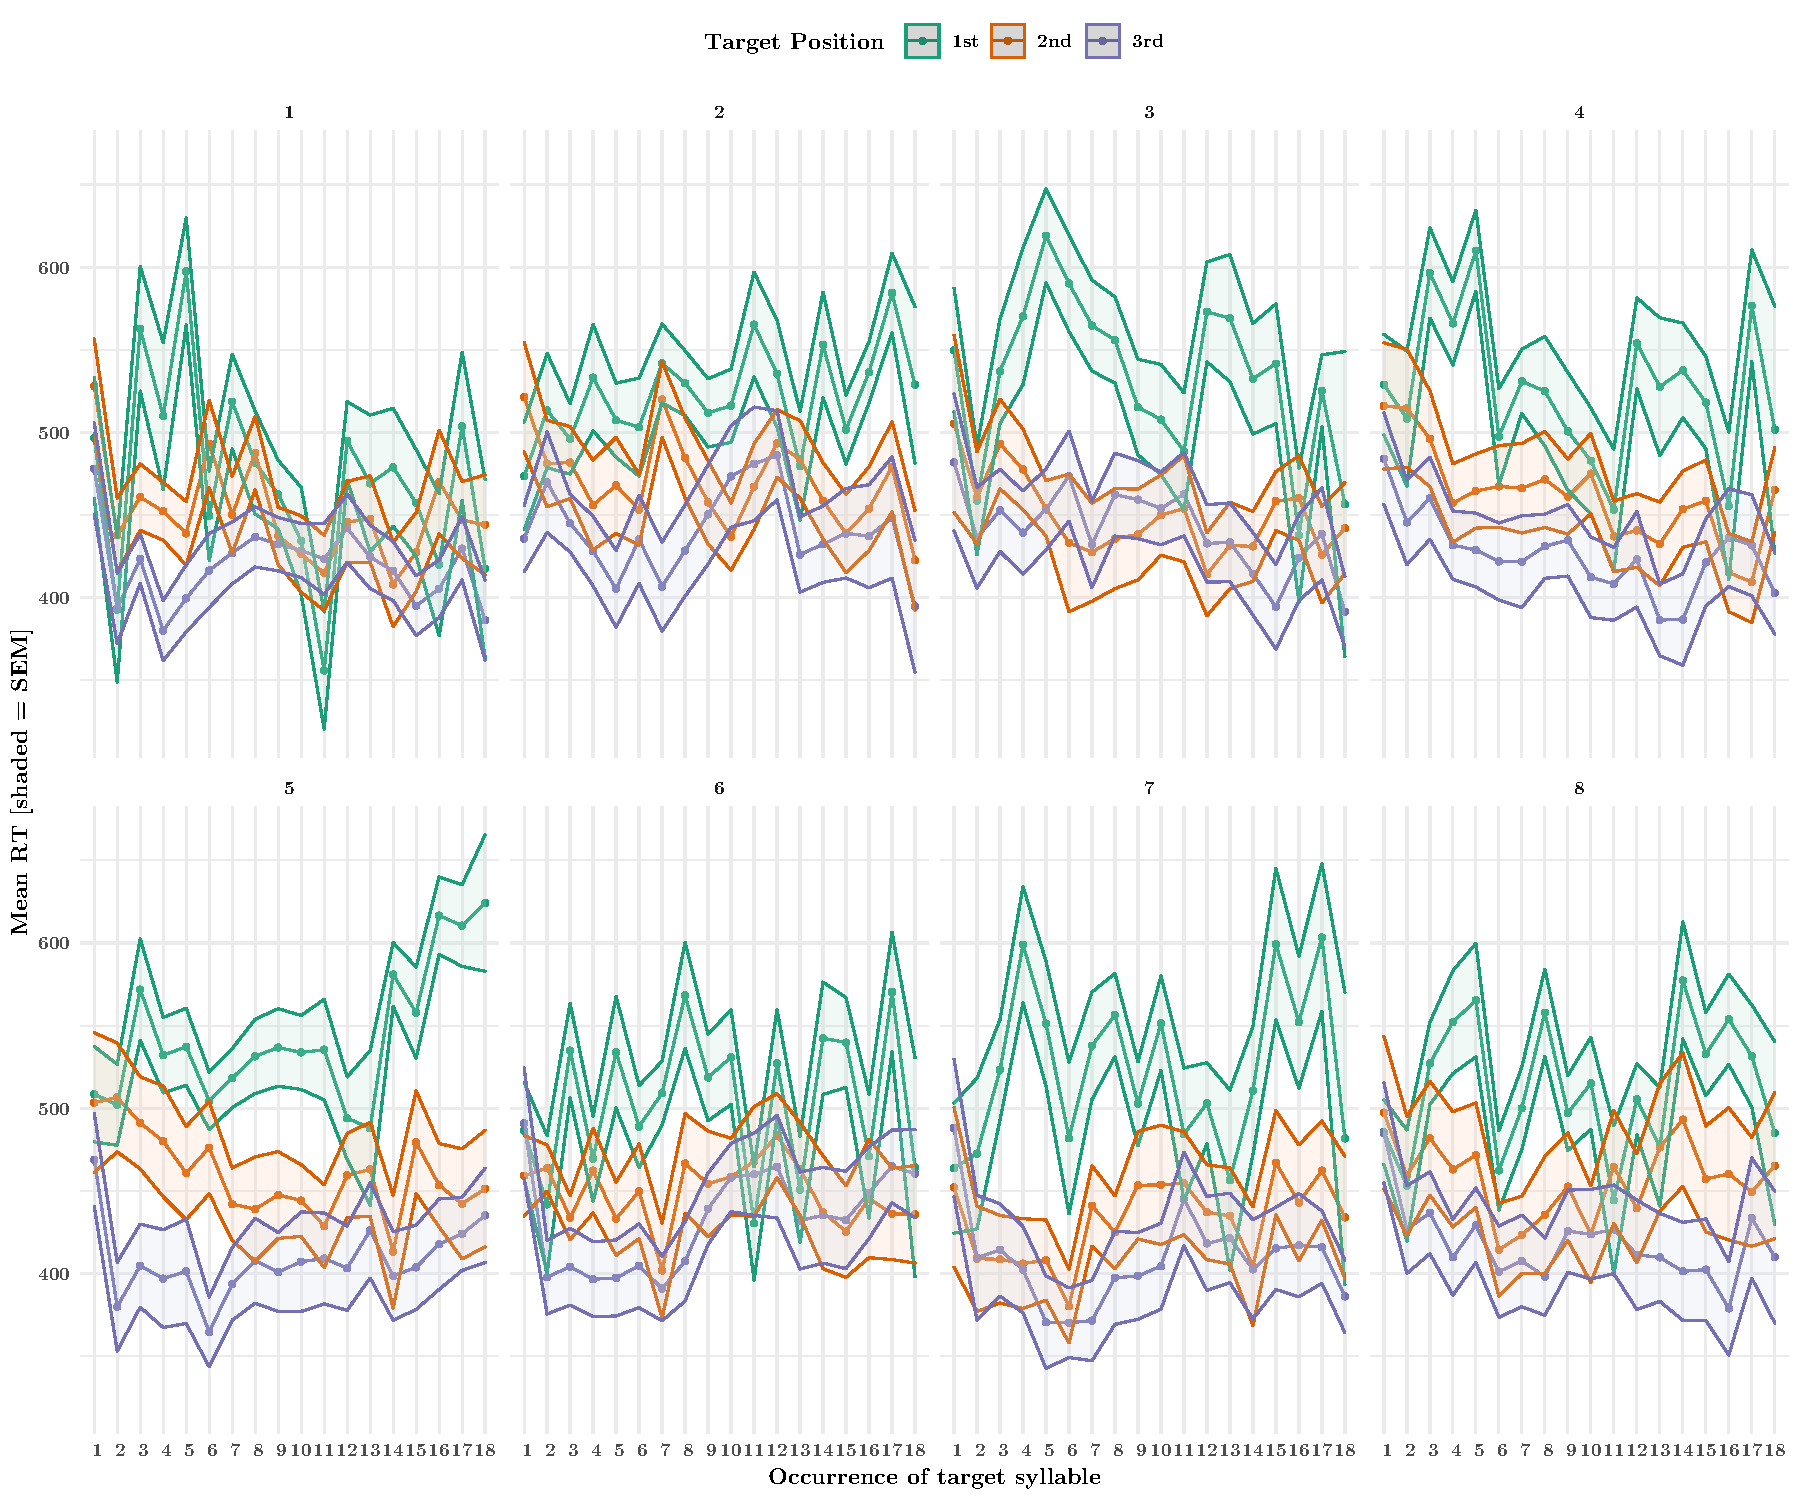
\includegraphics[width=0.8\textwidth]{exp3fig3brolling.pdf}
		\caption{Rolling means of reaction times in each block.}
		\end{subfigure}
		\begin{subfigure}{.4\textwidth}
		\centering
		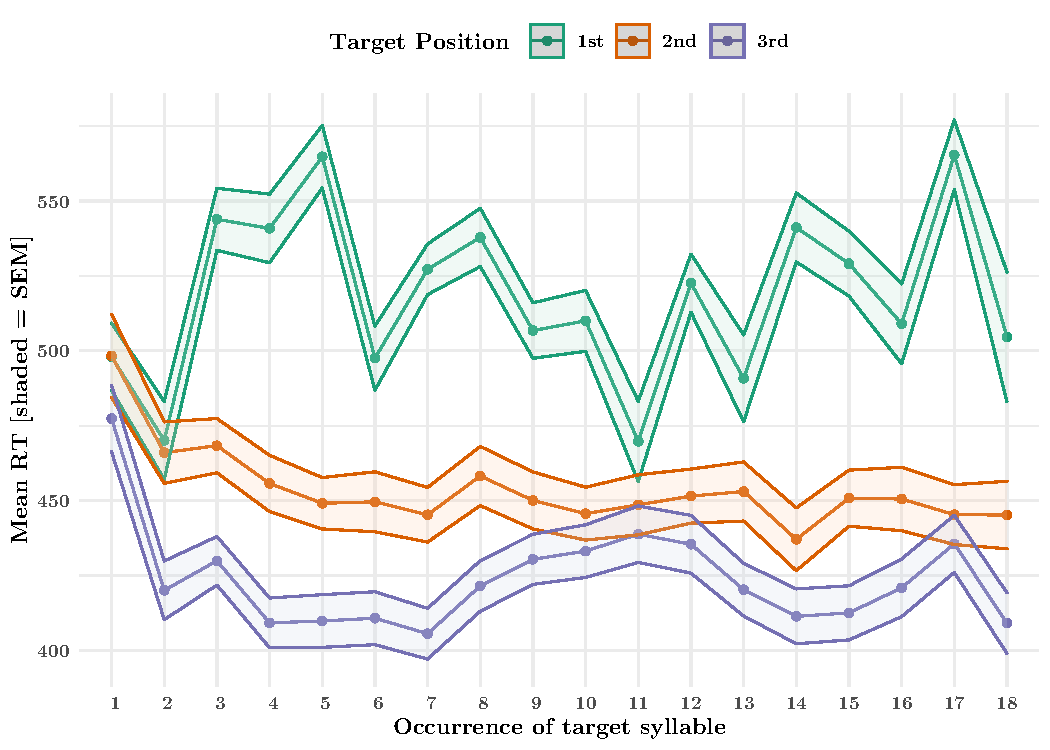
\includegraphics[width=\linewidth]{exp3fig3rolling.pdf}
		\caption{Grand averaged rolling means.}
	\end{subfigure}
	\label{fig:Fig. 2}
\end{figure}

\begin{figure}[H]
	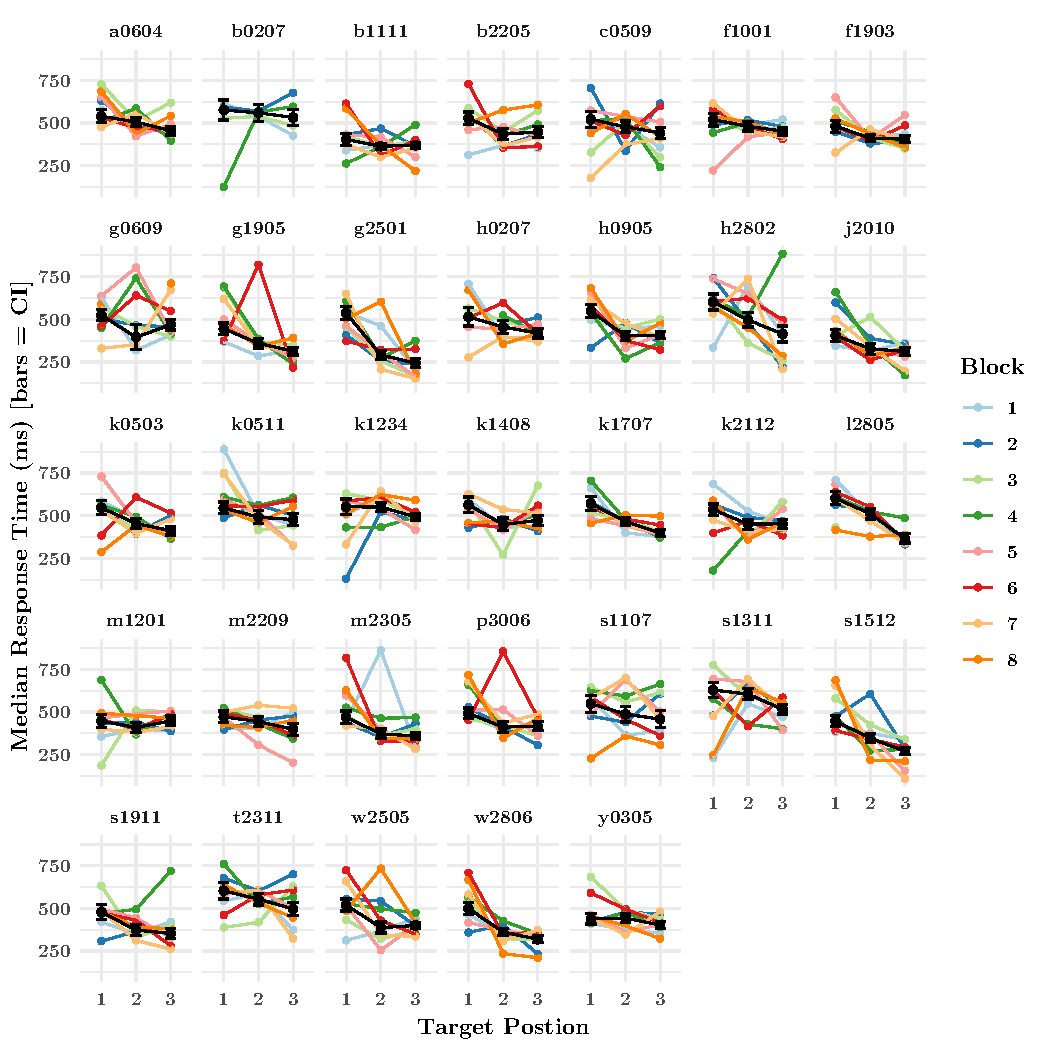
\includegraphics[width=\textwidth]{exp3fig2.pdf}
	\caption{Reaction times for each position in each participant.}
	\label{fig:Fig. 3}
\end{figure}




\begin{table}[!h] 
	\centering
	\caption{GLM Results} 
	\label{table:Table 2} 
	\resizebox{1.2\textwidth}{!}{
	\begin{tabular}{@{\extracolsep{2pt}}lD{.}{.}{-2} D{.}{.}{-2} D{.}{.}{-2} } 
		\\[-1.8ex]\hline 
		\hline \\[-1.8ex] 
		& \multicolumn{3}{c}{\textit{Dependent variable:}} \\ 
		\cline{2-4} 
		\\[-1.8ex] & \multicolumn{3}{c}{reaction time (s)} \\ 
		& \multicolumn{1}{c}{lesser} & \multicolumn{1}{c}{lesser (random slopes)} & \multicolumn{1}{c}{fuller} \\ 
		\\[-1.8ex] & \multicolumn{1}{c}{(1)} & \multicolumn{1}{c}{(2)} & \multicolumn{1}{c}{(3)}\\ 
		\hline \\[-1.8ex] 
		Intercept(Pos 1) & -0.63^{***}$ $(-0.68$, $-0.57) & -0.64^{***}$ $(-0.68$, $-0.61) & -0.69^{***}$ $(-0.76$, $-0.62) \\ 
		Pos 2 & -0.16^{***}$ $(-0.18$, $-0.14) & -0.14^{***}$ $(-0.19$, $-0.10) & -0.11^{***}$ $(-0.17$, $-0.05) \\ 
		Pos 3 & -0.23^{***}$ $(-0.25$, $-0.21) & -0.22^{***}$ $(-0.28$, $-0.15) & -0.18^{***}$ $(-0.24$, $-0.12) \\ 
		Block 2 &  &  & 0.07^{**}$ $(0.01$, $0.13) \\ 
		Block 3 &  &  & 0.08^{***}$ $(0.02$, $0.15) \\ 
		Block 4 &  &  & 0.08^{**}$ $(0.02$, $0.14) \\ 
		Block 5 &  &  & 0.11^{***}$ $(0.05$, $0.17) \\ 
		Block 6 &  &  & 0.03$ $(-0.03$, $0.09) \\ 
		Block 7 &  &  & 0.05$ $(-0.01$, $0.11) \\ 
		Block 8 &  &  & 0.06^{*}$ $(-0.005$, $0.12) \\ 
		Pos 2:Block 2 &  &  & -0.04$ $(-0.12$, $0.04) \\ 
		Pos 3:Block 2 &  &  & -0.03$ $(-0.11$, $0.05) \\ 
		Pos 2:Block 3 &  &  & -0.07^{*}$ $(-0.16$, $0.01) \\ 
		Pos 3:Block 3 &  &  & -0.03$ $(-0.11$, $0.05) \\ 
		Pos 2:Block 4 &  &  & -0.05$ $(-0.13$, $0.04) \\ 
		Pos 3:Block 4 &  &  & -0.07$ $(-0.15$, $0.01) \\ 
		Pos 2:Block 5 &  &  & -0.06$ $(-0.14$, $0.03) \\ 
		Pos 3:Block 5 &  &  & -0.14^{***}$ $(-0.22$, $-0.06) \\ 
		Pos 2:Block 6 &  &  & -0.01$ $(-0.10$, $0.07) \\ 
		Pos 3:Block 6 &  &  & 0.01$ $(-0.06$, $0.09) \\ 
		Pos 2:Block 7 &  &  & -0.06$ $(-0.15$, $0.02) \\ 
		Pos 3:Block 7 &  &  & -0.09^{**}$ $(-0.17$, $-0.004) \\ 
		Pos 2:Block 8 &  &  & -0.06$ $(-0.14$, $0.03) \\ 
		Pos 3:Block 8 &  &  & -0.06$ $(-0.14$, $0.02) \\ 
		\hline \\[-1.8ex] 
		Fixed Effects & Subject & Position | Subject & Subject \\ 
		Fixed Effects Struct. & Rand. Int. & Rand. Int., Slope & Rand Int. \\ 
		Observations & \multicolumn{1}{c}{9,531} & \multicolumn{1}{c}{9,531} & \multicolumn{1}{c}{9,531} \\ 
		Log Likelihood & \multicolumn{1}{c}{3,199.61} & \multicolumn{1}{c}{3,312.13} & \multicolumn{1}{c}{3,224.15} \\ 
		Akaike Inf. Crit. & \multicolumn{1}{c}{-6,389.23} & \multicolumn{1}{c}{-6,604.26} & \multicolumn{1}{c}{-6,396.29} \\ 
		Bayesian Inf. Crit. & \multicolumn{1}{c}{-6,353.42} & \multicolumn{1}{c}{-6,532.64} & \multicolumn{1}{c}{-6,210.07} \\ 
		\hline 
		\hline \\[-1.8ex] 
		\textit{Note:}  & \multicolumn{3}{r}{$^{*}$p$<$0.1; $^{**}$p$<$0.05; $^{***}$p$<$0.01} \\ 
		& \multicolumn{3}{r}{Fitted using Gamma distribution and log link function.} \\ 
	\end{tabular}} 
\end{table} 


\section{Experiment 2}
\subsection{Method}


\subsection{Results}





\section{Supplementary Materials}


\begin{figure}
	\begin{subfigure}{0.2\textwidth}
		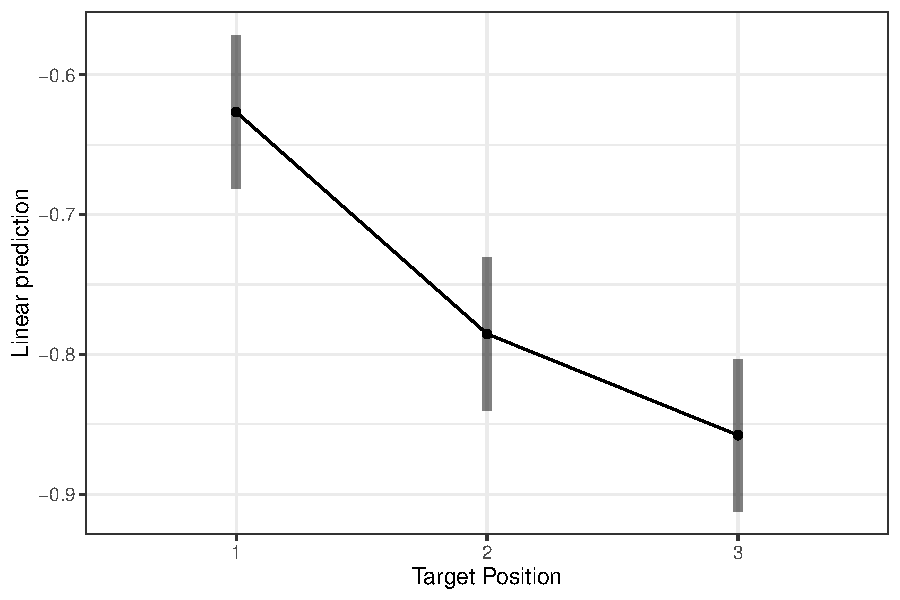
\includegraphics[width=0.3\textwidth]{exp3figS1.pdf}
		\caption{Predictions from linear model, with only position as predictor.}
	\end{subfigure} 
	\begin{subfigure}{\textwidth}
		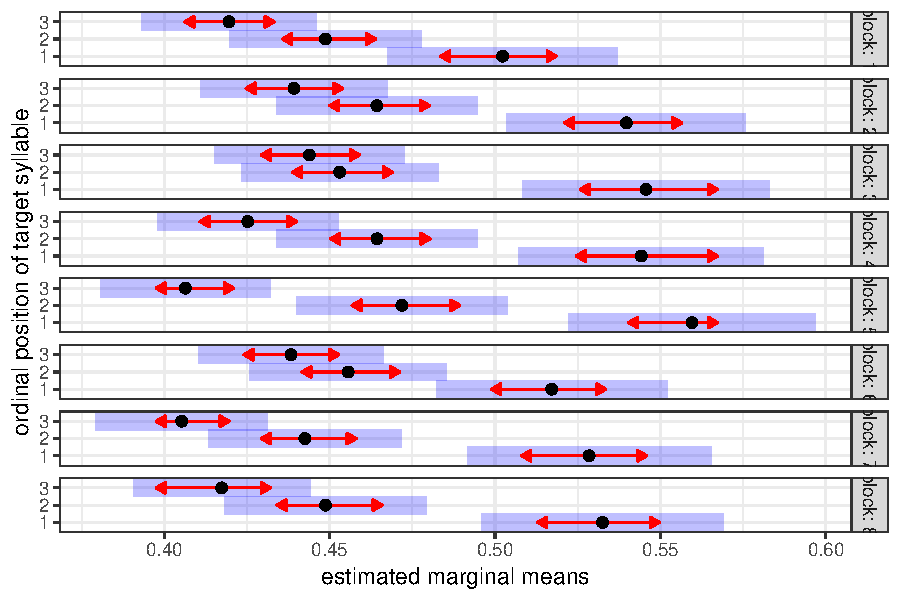
\includegraphics[width=0.3\textwidth]{exp3figS2a.pdf}
		\caption{Estimated means and contrasts from linear model with position and block as predictors.}
	\end{subfigure}
	\begin{subfigure}{\textwidth}
	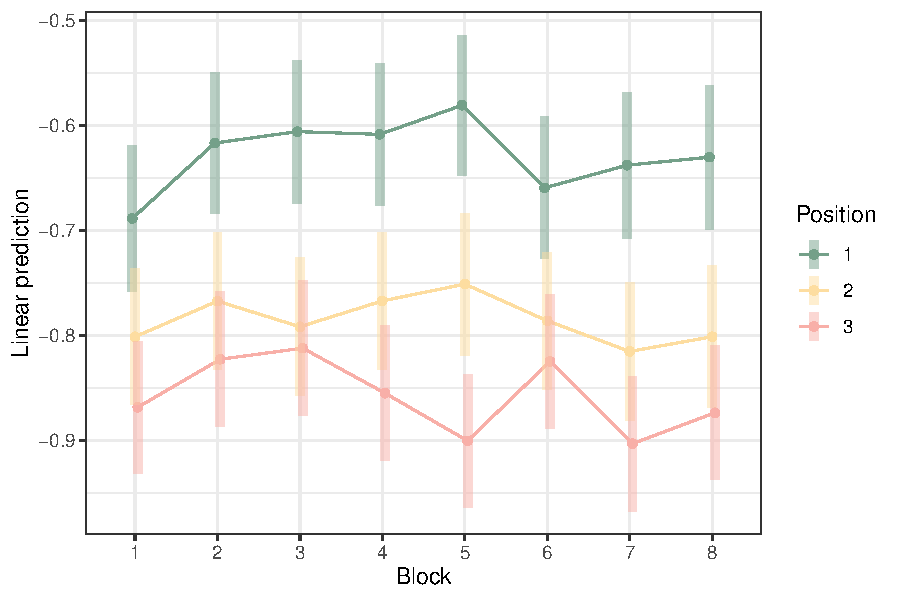
\includegraphics[width=0.3\textwidth]{exp3figS2b.pdf}
	\caption{Predictions from linear model, with position and block as predictors.}
	\end{subfigure}
	\label{fig:Fig. S1}
\end{figure}


\begin{figure}
	\begin{subfigure}{\textwidth}
		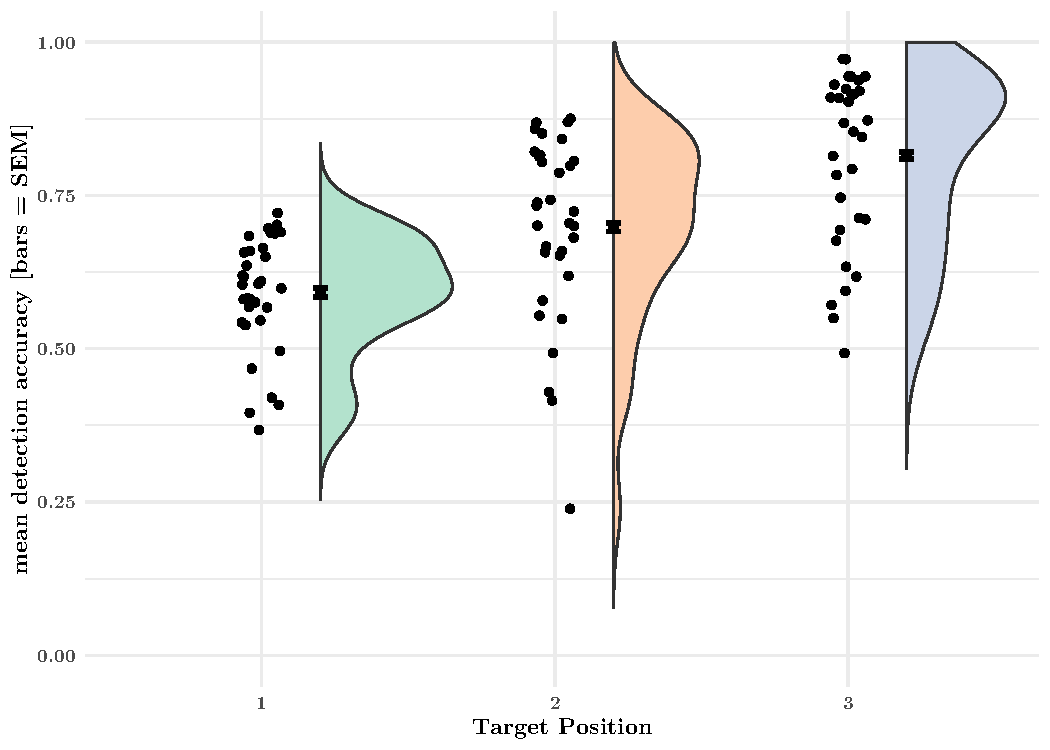
\includegraphics[width=0.4\textwidth]{exp3fig4acc.pdf}
		\caption{Accuracy for Experiment 1}
	\end{subfigure} 
	\begin{subfigure}{\textwidth}
		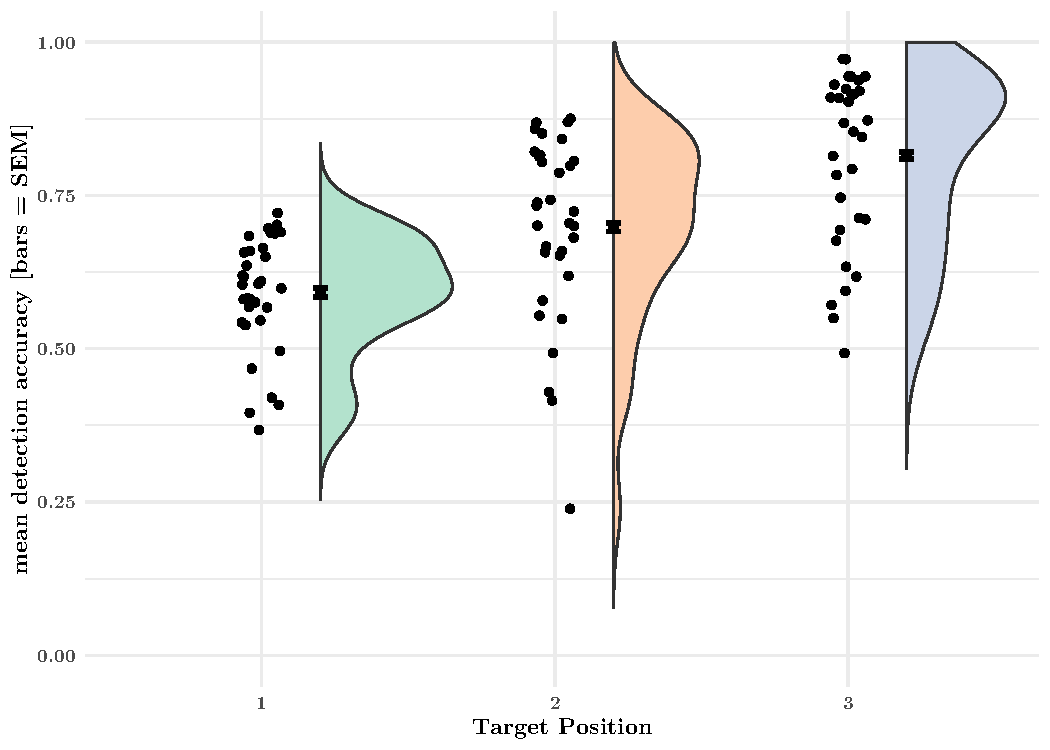
\includegraphics[width=0.4\textwidth]{exp3fig4acc.pdf}
		\caption{Accuracy for Experiment 2}
	\end{subfigure}
	\label{fig:Fig. S2}
\end{figure}
We quantified accuracy in the target detection task to ensure participants complied
with task instructions. The hit rate in Experiment 1 was 0.70 (\textit{sd} = 0.45). 
The hit rate was also modulated by ordinal position, with each successive position
having a higher mean accuracy (\textit{M\_{Pos 1}} = 0.59, \textit{sd\_{Pos 1}} = 0.49;
\textit{M\_{Pos 2}} = 0.70, \textit{sd\_{Pos 2}} = 0.46; \textit{M\_{Pos 3}} = 0.82, \textit{sd\_{Pos 3}} = 0.39) (~\ref{fig:Fig. S2}(a)).
When averaging across all syllables in a pseudoword, accuracy varied between the 
four words. This effect appears to be driven by differences in recognizibility of
individual syllables; certain CV syllable pairs may have been easier to detect
than others, due to minor variations in stimuli acoustics (~\ref{fig:Fig. S3}). 

\begin{figure}
	\begin{subfigure}{\textwidth}
		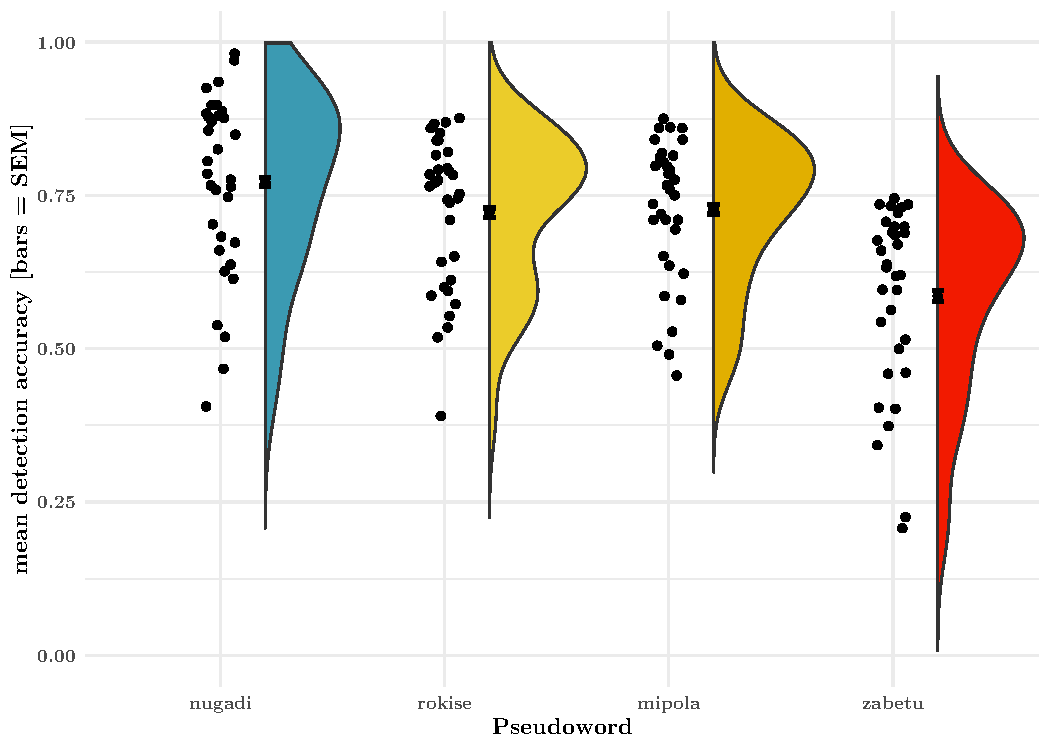
\includegraphics[width=0.5\textwidth]{exp3fig4bacc.pdf}
		\caption{Exp. 1, Accuracy by Word}
	\end{subfigure} 
	\begin{subfigure}{\textwidth}
		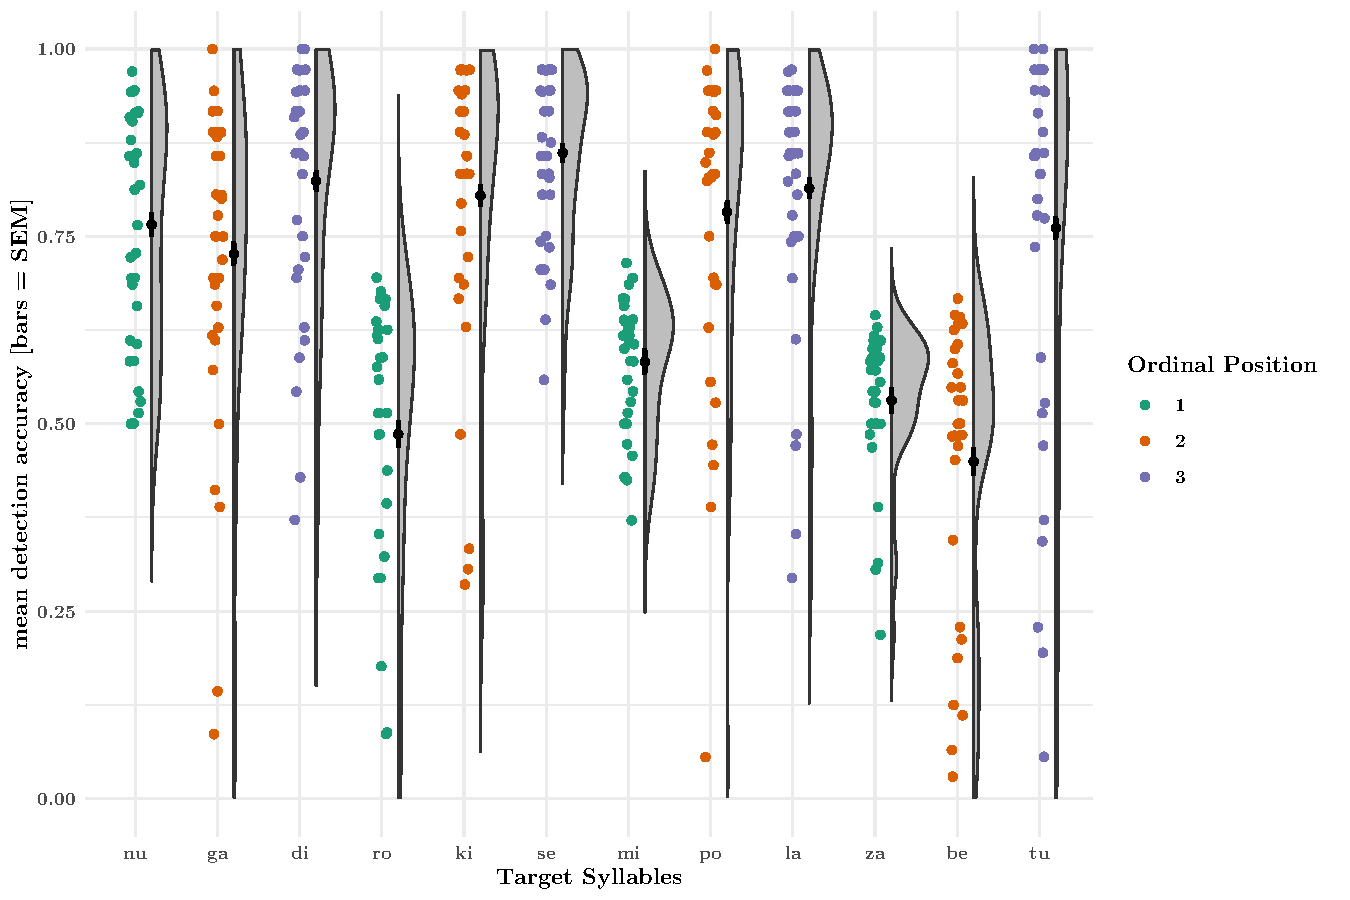
\includegraphics[width=0.5\textwidth]{exp3fig4cacc.pdf}
		\caption{Exp. 1, Accuracy by Syllable}
	\end{subfigure}
	\label{fig:Fig. S3}
\end{figure}



\addcontentsline{toc}{section}{References}
%\bibliographystyle{authoryear}
%\bibliography{library.bib}
\printbibliography[heading=bibintoc,title={References}]
\end{document}
